% Chapter mq, part C: denominators of CM formal groups, the splitting of (M), the Hankel product, hypothesis (B4) for the lemniscatic curve. Sources: misc/reviews/nick-arithmetic-geometry-M/arithmetic_geometry_M_for_vadim/chapter_arithmetic_geometry_M.tex, referee reports misc/research/directions/opus/vol3/MAG.md and misc/research/directions/astra/MAGA/report.md, numbers misc/vol3/verify/MAG/results.md; revised 23 Nov 2026 after MQ_review.md and MQA/report.md.
\section{Arithmetic geometry and the inequality (M): what survives}\label{mqg:sec:ag}

This part collects the arithmetic results that survive the refereeing of an attempt to prove the inequality (M) of Part A by arithmetic geometry (slope inequalities for formal groups of CM elliptic curves). The attempt does not prove (M). What it gives is an exact description of the denominators of the logarithm of a CM formal group as a Chebyshev function of the CM field, a decomposition of the statistic into an integer and a sign, a closed form for a family of Hankel determinants, and a proof of a local integrality statement. Most ingredients are classical, and we attribute them. For a function $w$ on prime powers write $\psi_w(n)=\sum_{p^k\le n}w(p^k)\log p$, and $\chi_d$ for the Kronecker character of $\mathbb Q(\sqrt{-d})$, of discriminant $-d$ (so $\chi_4$ belongs to $\mathbb Q(i)$). As in Part A, $\chi_q$ is the real primitive character of discriminant $-q$, so that $\chi_q\chi_d=\chi_{qd}$ has discriminant $+qd$, and the weights of (M) are as there. The integer determinants, valuations and denominators quoted were computed in exact arithmetic, the logarithmic shares and the extrema of the sign plots in floating point.

\subsection{The denominator theorem}\label{mqg:sec:denom}

Let $E$ be an elliptic curve over $\mathbb Q$ with complex multiplication by $\mathbb Q(\sqrt{-d})$ and $L(E,s)=\sum a_nn^{-s}$. A prime is good if $E$ has good reduction there. A good prime is unramified in the CM field (a ramified prime is a prime of additive reduction), so it splits or is inert. By the theory of complex multiplication (Deuring), $L(E,s)$ is the $L$ function of a Hecke character of the CM field, hence $a_p$ is a unit at a split good prime, and $a_p=0$ at an inert one. For a good prime $p$ the recurrence $a_{p^{j+1}}=a_pa_{p^j}-pa_{p^{j-1}}$ gives $a_{p^j}\equiv a_p^j\pmod p$ at a split prime, and $a_{p^{2i}}=(-p)^i$, $a_{p^{2i+1}}=0$ at an inert prime. The formal group of $E$ at a good prime has the logarithm $\sum a_nx^n/n$ up to an isomorphism with unit linear term (Honda \cite{Honda70}). Such an isomorphism over $\mathbb Z_p$ has an integral inverse and mixes only coefficients of degree at most $n$ in each direction, so it does not change the least common denominator of the coefficients of degree at most $n$.

\begin{theorem}[denominators of a CM logarithm]\label{mqg:thm:lcmgen}
Let $\mathcal D_n$ be the least common denominator of the numbers $a_k/k$, $k\le n$, taken over the good primes only. Then $v_p(\mathcal D_n)=\lfloor\log_pn\rfloor$ at a split good prime and $\lfloor\log_{p^2}n\rfloor$ at an inert good prime. Consequently
\[
2\log\mathcal D_n=\psi_{1+\chi_d}(n),\qquad\psi_{1-\chi_d}(n)=2\log\frac{\mathrm{lcm}(1,\dots,n)}{\mathcal D_n},
\]
where $\psi_{1\pm\chi_d}$ and $\mathrm{lcm}(1,\dots,n)$ are both restricted to the good primes.
\end{theorem}

\begin{proof}
Write $k=p^jr$ with $p\nmid r$. By multiplicativity $a_k=a_{p^j}\prod a_{q^i}$ over the other prime powers exactly dividing $k$, and these factors are integers, so $v_p(a_k/k)\ge v_p(a_{p^j}/p^j)$. Hence the denominator at $p$ is maximal already at a pure power $p^j\le n$. At a split prime $a_{p^j}$ is a unit, so the denominator of $a_{p^j}/p^j$ is $p^j$ and $v_p(\mathcal D_n)=\lfloor\log_pn\rfloor$. At an inert prime the odd powers give $0$ and $a_{p^{2i}}/p^{2i}=\pm p^{-i}$, so $v_p(\mathcal D_n)=\max\{i:p^{2i}\le n\}$. Since $(1+\chi_d(p^k))/2$ is $1$ at every power of a split prime, $1$ at even and $0$ at odd powers of an inert prime, this is the stated value of $2\log\mathcal D_n$. The second identity follows because $\mathrm{lcm}(1,\dots,n)$ has $v_p=\lfloor\log_pn\rfloor$ and $1-\chi_d=2-(1+\chi_d)$.
\end{proof}

The theorem concerns a curve over $\mathbb Q$ with complex multiplication, so the CM field has class number one. Every $d$ admissible for (M) has class number greater than one (Subsection~\ref{mql:sub:general} of Part B). Applying the construction to the fields of (M) therefore needs a larger field of definition, its integral models, a norm, and archimedean estimates at all embeddings.

The restriction to good primes is needed. At a bad prime $a_{p^k}=0$, so $v_p(\mathcal D_n)=0$ while the lcm has $\lfloor\log_pn\rfloor$. A fixed finite set of bad primes contributes $O(\log n)$ to either raw side, so the restriction does not change the size of the statistic, though a linear centring of a smoothed sum changes separately. At $p=2$ the theorem applies only when $2$ is good, as it is for $49a1$.

\textbf{Checks.} For the curves $y^2=x^3-x$ ($d=4$) and $49a1$ ($d=7$) the valuations of $\mathcal D_n$ equal the predicted ones for every good odd prime and every power $p^j\le10^5$ (9591 odd primes for $d=4$, 9590 for $d=7$), so $2\log\mathcal D_n=\psi_{1+\chi_d}(n)$ holds for all $n\le10^5$ over the odd good primes.

\subsection{The lemniscatic case}\label{mqg:sec:lemn}

For $d=4$ the logarithm of the formal group of $y^2=x^3-x$ is $\mathrm{arcsl}(s)=\int_0^s(1-t^4)^{-1/2}dt=\sum_{j\ge0}\lambda_js^{4j+1}$ with $\lambda_j=\binom{2j}{j}/(4^j(4j+1))$. Let $\Lambda_n$ be the odd part of the least common denominator of the $\lambda_j$ with $4j+1\le n$. Theorem~\ref{mqg:thm:lcmgen} gives the odd part of the following for $d=4$ up to an isomorphism of formal groups; the elementary proof below does not need that, nor any statement about height.

\begin{theorem}[the lemniscatic denominators]\label{mqg:thm:lemn}
For every odd prime $p$, $v_p(\Lambda_n)=\lfloor\log_pn\rfloor$ if $p\equiv1\pmod4$ and $\lfloor\log_{p^2}n\rfloor$ if $p\equiv3\pmod4$. Hence, with all sums over odd primes,
\[
2\log\Lambda_n=\psi_{1+\chi_4}(n),\qquad2\log\frac{\mathrm{lcm}(1,\dots,n)_{\rm odd}}{\Lambda_n}=\psi_{1-\chi_4}(n).
\]
\end{theorem}

\begin{proof}
The $p$ part of the denominator of $\lambda_j$ is $p^{e-v_p\binom{2j}{j}}$ with $e=v_p(4j+1)$, when this exponent is positive. At $p\equiv1\pmod4$ the exponent is at most $e\le\log_p(4j+1)$. At $p\equiv3\pmod4$ it is at most $\lfloor e/2\rfloor$ by the carry lemma of Part B, which we recall. If $p^e$ exactly divides $4j+1$ then $j\equiv-\frac14\pmod{p^e}$. Since $-\frac14=\frac{(p^2-1)/4}{1-p^2}$ and $\frac{p^2-1}{4}=\frac{3p-1}{4}+p\,\frac{p-3}{4}$, the $p$ adic digits of $-\frac14$ repeat with period two, least significant first: $\frac{3p-1}{4},\frac{p-3}{4}$. In the sum $j+j$ the digit $\frac{3p-1}{4}$ produces a carry, and the digit $\frac{p-3}{4}$ with the incoming carry gives $\frac{p-1}{2}<p$ and does not. So the first $e$ digits give $\lceil e/2\rceil$ carries, and by Kummer's theorem $v_p\binom{2j}{j}\ge\lceil e/2\rceil$. The exponent is therefore at most $\lfloor e/2\rfloor\le\lfloor\log_{p^2}(4j+1)\rfloor$.

Attainment. For $p\equiv1\pmod4$ and $4j+1=p^k$ the base $p$ digits of $j=(p^k-1)/4$ are all $\frac{p-1}{4}$, there is no carry in $j+j$, and the exponent is $k$. For $p\equiv3\pmod4$ and $4j+1=p^{2k}$ the digits of $j$ are $k$ repetitions of the pair $\frac{3p-1}{4},\frac{p-3}{4}$, giving exactly $k$ carries and the exponent $2k-k=k$. The values of $\psi_{1\pm\chi_4}$ follow as in the previous proof.
\end{proof}

\textbf{Checks.} The valuations agree with the formulae for all $782$ odd primes up to $n=6001$.

\textbf{Reading.} The first identity says that $e^{\psi_{1+\chi_d}(n)/2}$ is the denominator of the logarithm of the CM formal group, as $\mathrm{lcm}(1,\dots,n)=e^{\psi(n)}$ is that of $\mathbb G_m$. Thus the weight $1-\chi_d$ of (M) is, up to the bad primes, twice the logarithm of the integer $\mathrm{lcm}(1,\dots,n)/\mathcal D_n$, and an upper bound for the Riesz mean of $\psi_{1-\chi_d}$ is a statement on average about the index of two integral structures, not a pointwise bound (see the warnings after Theorem~\ref{mqg:thm:splitting}).

\subsection{Twists, and the integer plus sign decomposition}\label{mqg:sec:twist}

\begin{proposition}[twists have the same denominators]\label{mqg:prop:twist}
Let $\chi$ be a quadratic character of conductor prime to the bad primes. At every good prime not dividing the conductor, the series $\sum\chi(n)a_nx^n/n$ has the same least common denominators $\mathcal D_n$ as $\sum a_nx^n/n$, and $\sum\chi(n)x^n/n$ has those of $\sum x^n/n$.
\end{proposition}

\begin{proof}
$\chi(p^j)=\pm1$ does not change $v_p(a_{p^j}/p^j)$, and terms with $\chi(k)=0$ cannot raise a maximum already attained at a pure prime power.
\end{proof}

So no quotient of the denominators of the logarithms of the curve, of $\mathbb G_m$, or of their quadratic twists, can produce the factor $1+\chi_q$ of (M). A twist multiplies the Frobenius eigenvalue by the sign $\chi_q(p)$ and leaves the height alone, and denominators see heights. Expanding the weight, and writing $\chi_q$ for the character of the second field of (M),
\begin{equation}\label{mqg:eq:split}
\psi_{(1+\chi_q)(1-\chi_d)}(n)=\underbrace{2\log\frac{\mathrm{lcm}(1,\dots,n)}{\mathcal D_n}}_{\text{twice the log of an integer}}+\underbrace{\psi_{\chi_q}(n)-\psi_{\chi_q\chi_d}(n)}_{\text{a sum of signs}},
\end{equation}
all over the good primes. The second term equals $2\sum\chi_q(p)\log p$ over the odd prime powers $p^k$ of inert primes (for even $k$ the factor $1-\chi_d(p^k)$ vanishes), and ramified primes have sign zero. The first term has main term $n$, the second none. At a prime ramified in the CM field, such as $7$ for $d=7$, $\chi_d$ vanishes while the signed weight need not, so restoring it adds $(-1)^j\log7$ at $7^j$; this is the dependence on the convention at the prime $7$ noted below.

For $q=11$, $d=7$ and $100\le n\le4\cdot10^6$, without smoothing, with the prime $7$ given weight one in the first term and $\chi_q(p)=(p/11)$ in the second, the ranges of the quantities divided by $\sqrt n$ are $[-1.81,1.76]$ for the first term minus $n$, $[-3.59,4.23]$ for the second term, and $[-4.83,5.59]$ for their sum. All six extremes occur below $10^5$. These are floating point computations, and the ranges depend on the convention at the prime $7$ (weight two gives $[-4.79,5.75]$ for the sum, removing it $[-4.87,5.48]$). Both parts are of square root size in this range, as GRH predicts, an observation on a finite range only.

\begin{figure}[htbp]
\centering
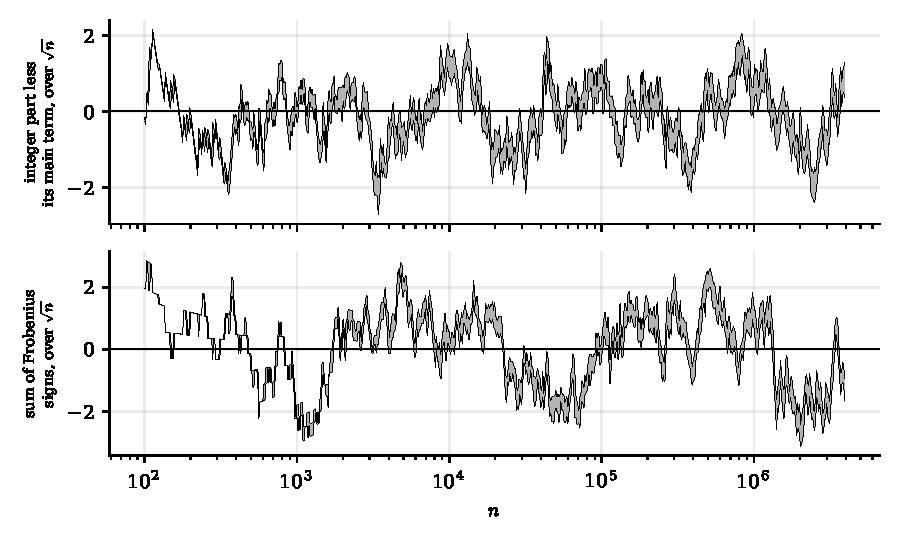
\includegraphics[width=0.95\textwidth]{fig/mq_integer_sign.pdf}
\caption{The two parts of the statistic of (M) for $(q,d)=(3,23)$, divided by $\sqrt n$, without smoothing, for $100\le n\le4\cdot10^6$ (numerical; good primes only): the integer part $2\log(\mathrm{lcm}(1,\dots,n)/\mathcal D_n)$ less its main term $n$ (top) and the sum of Frobenius signs (bottom), shown as the least and greatest value in each logarithmic bin.}\label{mqg:fig:integersign}
\end{figure}

Figure~\ref{mqg:fig:integersign} shows the two terms of equation~\eqref{mqg:eq:split} for the admissible pair $(3,23)$: the integer part less $n$ lies in $[-2.72,2.16]$ (its extreme is at $n=3448$) and the sign part in $[-3.12,2.85]$ (its extreme is at $n=2049521$), and the sum in $[-4.75,4.44]$, all divided by $\sqrt n$.

The decomposition separates two difficulties. The first term asks for control, in the mean sense of the statistic, of the size of an explicit integer. The second asks for cancellation in a sum of Frobenius signs over the inert primes, of the kind of the Chebotarev theorem with a power saving. We know no mechanism for the second except to control the zeros of $L(s,\chi_q)$ and $L(s,\chi_q\chi_d)$. The sign part is, up to local corrections at the excluded primes, minus the logarithmic derivative of $L(s,\chi_q)/L(s,\chi_q\chi_d)$, not that of the $L$ function of the twisted curve, which has degree two.

\subsection{Splitting a fixed character bound}\label{mqg:sec:split}

Let $\mathcal R$ be the Riesz mean $\mathcal Rf(x)=x\int_1^xf(t)t^{-2}dt$, so that the fixed character statistic of this subsection is $\mathcal R\psi_w$ (Proposition~\ref{qt:prop:riesz} for the unweighted case). This is an analytic bound for fixed characters and globally bounded means. It is not (M), which has moving windows and a frame budget, and (M) is not deduced from it. Fix the real primitive characters $\chi_q,\chi_d$ of distinct discriminants $-q,-d$, so that all three characters $\chi_q,\chi_d,\chi_{qd}$ are nonprincipal. Fix a finite set $S_0$ of excluded primes (the bad primes), and let $\Lambda_S$ be the von Mangoldt function restricted to prime powers outside $S_0$. Put
\[
D_1(s)=\sum_n(1-\chi_d(n))\Lambda_S(n)n^{-s},\qquad D_2(s)=\sum_n\chi_q(n)(1-\chi_d(n))\Lambda_S(n)n^{-s},
\]
and let $P_1,P_2$ be the Riesz means of the corresponding partial sums. Their Mellin transforms on $\Re s>1$ are $D_j(s)/(s(s-1))$. Write $D_1(s)=\frac1{s-1}+b_1+O(s-1)$ and $D_2(s)=b_2+O(s-1)$. The main terms are
\[
M_1(x)=x\log x+(b_1-1)x,\qquad M_2(x)=b_2x.
\]
The constants $b_1,b_2$ depend on $S_0$. The pole of $D_2$ at $s=1$ is absent, and $b_2x$ comes from the smoothing kernel, so $b_2$ may in principle vanish.

\begin{theorem}[splitting of a fixed character analytic bound]\label{mqg:thm:splitting}
Assume the following.
\begin{enumerate}
\item[(R)] $L(s,\chi_d)$ and $L(s,\chi_q\chi_d)$ have no real zero in $(\frac12,1)$.
\item[(NC)] (no conspiracy) For every $\rho$ with $\Re\rho>\frac12$ that is a zero of one of the four functions $\zeta$, $L(\chi_q)$, $L(\chi_d)$, $L(\chi_q\chi_d)$, the signed sum of multiplicities $m_\zeta(\rho)+m_{\chi_q}(\rho)-m_{\chi_d}(\rho)-m_{\chi_q\chi_d}(\rho)$ is nonzero.
\end{enumerate}
Then the following are equivalent.
\begin{enumerate}
\item[(a)] $P_1(x)+P_2(x)\le M_1(x)+M_2(x)+O_\varepsilon(x^{1/2+\varepsilon})$ for every $\varepsilon>0$.
\item[(b)] Both bounds $P_1\le M_1+O_\varepsilon(x^{1/2+\varepsilon})$ and $P_2\le M_2+O_\varepsilon(x^{1/2+\varepsilon})$ hold.
\item[(c)] $\zeta$, $L(\chi_d)$, $L(\chi_q)$, $L(\chi_q\chi_d)$ have no zero with $\Re s>\frac12$.
\end{enumerate}
The directions (c) $\Rightarrow$ (b) $\Rightarrow$ (a) need neither hypothesis. For the bound on $P_1$ alone, equivalent to RH for $\zeta$ and $L(\chi_d)$, it suffices to assume $L(\chi_d)$ has no real zero in $(\frac12,1)$ and $m_\zeta\ne m_{\chi_d}$ at the zeros in $\Re s>\frac12$. For $P_2$ alone, equivalent to RH for $L(\chi_q)$ and $L(\chi_q\chi_d)$, assume (R) for $L(\chi_q\chi_d)$ and $m_{\chi_q}\ne m_{\chi_q\chi_d}$ there.
\end{theorem}

\begin{proof}
The implication (a) $\Rightarrow$ (c) is a consequence of the signed Landau proposition of Part A, Proposition~\ref{mq:prop:onesided}(1) (behind which is Landau's theorem \cite{Landau05} on the real singularity of the Mellin transform of a nonnegative function). It says: if $R(x)\le Cx^\theta$ for all large $x$ and no real $\beta\in(\theta,1)$ has negative net multiplicity $n(\beta)$, then $n(\rho)=0$ for every $\rho$ with $\Re\rho>\theta$. For (c) $\Rightarrow$ (b) the explicit formula of Ingham \cite{Ingham32} gives the error term, the zero weights being absolutely summable of order $(1+|\Im\rho|^2)^{-1}$ for fixed conductors, and the matched main terms are the pole terms. The implication (b) $\Rightarrow$ (a) is addition.

For (a) $\Rightarrow$ (c), fix $\theta=\frac12+\varepsilon$ and apply the proposition to $R=P_1+P_2-M_1-M_2$, whose net multiplicity at $\rho$ is $n(\rho)=m_\zeta+m_{\chi_q}-m_{\chi_d}-m_{\chi_q\chi_d}$ (the residue of the transform at $\rho$ is proportional to $n(\rho)/(\rho(1-\rho))$). Under (R) no real $\beta\in(\theta,1)$ has $n(\beta)<0$, so $n(\rho)=0$ for $\Re\rho>\theta$, and under (NC) there is then no zero there. Sign logic: a real zero $\beta\in(\frac12,1)$ of a function entering with a positive coefficient ($\zeta$, $L(\chi_q)$) contributes $+x^\beta/(\beta(1-\beta))$ to $P-M$ and would violate the upper bound, while one of a function entering with a negative coefficient ($L(\chi_d)$, $L(\chi_q\chi_d)$) pushes the statistic down and is invisible to an upper bound. This is why (R) is needed exactly for the latter two. Let $\varepsilon\to0$ and use the functional equations of the primitive factors; removing Euler factors adds zeros only on $\Re s=0$. The same argument with the two function versions gives the statements for $P_1$ and $P_2$ alone.
\end{proof}

Hypothesis (NC) is unproved, and since the four functions are the factors of the Dedekind zeta function of a biquadratic field, it is a statement about simple zeros. Two warnings. First, an upper bound for a Riesz mean of $\psi_{1-\chi_d}(n)=2\log(\mathrm{lcm}/\mathcal D_n)$ does not give the pointwise bound $\mathcal I_n\le\exp((n+C\sqrt n)/2)$ for the integer $\mathcal I_n=\mathrm{lcm}/\mathcal D_n$: with the correct centring, a pointwise upper bound for $2\log\mathcal I_n-n$ gives a lower bound for the centred mean, and a converse needs a Tauberian argument with a loss. Second, without any error term the prime number theorem in fixed progressions already gives $\log\mathcal I_n=n/2+o(n)$, which is a different statement from $\mathcal I_n\sim e^{n/2}$. The fixed character bounds are therefore as hard as zero free half planes for two $L$ functions, in the sense of the equivalence above.

\subsection{The Hankel determinants of the lemniscate sine}\label{mqg:sec:hankel}

Let $s=\mathrm{sl}$ be the lemniscate sine, $s'^2=1-s^4$, $s''=-2s^3$. Write $D=d/dz$ and put $\mu_j=(D^{4j+1}s)(0)$, so that $\mu_0,\mu_1,\mu_2,\mu_3,\mu_4=1,-12,3024,-4390848,21224560896$, and $H_m=\det(\mu_{i+j})_{0\le i,j<m}$.

\begin{theorem}[closed form]\label{mqg:thm:hankel}
For $m\ge1$, $H_m=\prod_{k=1}^{m-1}q_k^{\,m-k}$ with $q_k=(4k-3)(4k-2)^2(4k-1)^2(4k)^2(4k+1)$.
\end{theorem}

This is classical: it is the Stieltjes and Rogers continued fraction for the Jacobi function $\mathrm{sn}$ (Stieltjes, Rogers \cite{Rogers07}, Flajolet \cite{Flajolet80}) combined with the Heilermann formula for the Hankel determinants of a J fraction, as treated for the coefficients of $\mathrm{sn}$, $\mathrm{cn}$, $\mathrm{dn}$ by Milne \cite{Milne02}. A direct proof in our normalisation: with $B=D^2$ one has $Bs^r=r(r-1)s^{r-2}-r(r+1)s^{r+2}$. On the odd powers $s,s^3,\dots$ the matrix of $B$ has zero diagonal, and the product of the two entries across the $j$th edge, between $s^{2j-1}$ and $s^{2j+1}$, is $t_j=-(2j-1)(2j)^2(2j+1)$. The restriction of $B^2$ to $s,s^5,s^9,\dots$ is tridiagonal with integer diagonal, and the product of the entries across its $k$th edge, between $s^{4k-3}$ and $s^{4k+1}$, is $t_{2k-1}t_{2k}=q_k$ (for $k=1$, $(-12)(-240)=2880$). The moment $\mu_k$ is the coefficient of $s$ in $(B^2)^ks$. The three term recurrence diagonalises the Gram matrix of moments by an integral unit triangular change of basis with diagonal $h_0=1$, $h_j=q_1\cdots q_j$, and multiplying gives $H_m=\prod h_j$. We verified the formula exactly for every $m\le60$.

\begin{corollary}\label{mqg:cor:sym}
$H_m>0$ and every prime factor of $H_m$ is at most $4m-3$. For fixed odd $p$, $v_p(H_m)=4m^2/(p-1)+O_p(m\log m)$, and the same holds at $p=2$ since $v_2(q_k)=6+2v_2(k)$. The leading growth $4m^2/(p-1)$ is the same at inert and at split primes, but the determinants distinguish them at their first positive valuation: for $p\equiv1\pmod4$ the first factor $q_k$ divisible by $p$ is at $k=(p-1)/4$ (where $4k+1=p$), with exponent $1$, and for $p\equiv3\pmod4$ at $k=(p+1)/4$ (where $4k-1=p$), with exponent $2$. The same holds for the pivots $H_m/H_{m-1}=\prod_{k<m}q_k$ and for the Smith factors $h_j$, with $v_p(h_j)=8j/(p-1)+O_p(\log j)$.
\end{corollary}

\textbf{Observations.} At $m=200$ the ratios $v_p(H_m)/m^2$ for $p=3,5,7,11,13,17$ are $1.963,0.977,0.649,0.386,0.321,0.239$, against $4/(p-1)=2,1,0.667,0.4,0.333,0.25$. For $m=14$ the Smith valuations (increasing order) of the matrix $(\mu_{i+j})$ are the following, in agreement with the valuations of $h_0,\dots,h_{13}$.
\begin{center}
\begin{tabular}{ll}
\hline
$p=7$, inert & $0,0,2,2,4,5,6,8,8,10,10,12,14,16$\\
$p=13$, split & $0,0,0,1,2,2,2,4,4,4,6,6,6,8$\\
$p=5$, split & $0,1,2,4,6,8,10,12,14,16,18,19,20,24$\\
$p=3$, inert & $0,2,6,10,12,17,20,26,29,34,36,40,44,46$\\
\hline
\end{tabular}
\end{center}

A slope or determinant inequality of rank $m$ drawn from this lattice is therefore a statement about explicit integers that sees the character only in lower order terms and in the first valuation. This concerns these determinants and pivots only; it does not rule out a method that keeps single vectors of the lattice instead of its volume. An exact evaluation of such a determinant is elementary, and is not of the depth of (M).

Split primes can divide $\mu_j$: for $p<200$ and $j<500$ the prime $157$ divides $\mu_j$ for $j\equiv25\pmod{39}$ (13 values) and $181$ for $j\equiv26,41\pmod{45}$ (22 values). The Kummer congruence of Theorem~\ref{mql:thm:kummer} is classical (Hurwitz \cite{Hurwitz99} for the Hurwitz numbers). The statement that the matrix has small rank modulo a split prime, which one might hope to derive from the congruence, is not established here.

\begin{remark}[slope inequalities]\label{mqg:rem:bost}
The slope method rests on Bost's slope inequality for filtered lattices \cite{Bost95,Bost01}. We use it only qualitatively. One naive integral version fails: for the point $P=(0,1)$ of the quartic model $w^2=1-s^4$ and the function $F=w-1$, which vanishes to order $T=4$, the leading jet is $-12$, not divisible by $4!=24$, because $w=1-s^4/2+\cdots$ has the prime $2$ in its coefficients. For odd primes the integrality needed for the inert prime bound does hold. So a factorial divisibility assertion for an integral auxiliary function fails on this curve.
\end{remark}

\begin{remark}[the integral method]\label{mqg:rem:integral}
Write $\lambda_j=\mathbb E[(S^2U)^{2j}]$ with $S$ uniform on $[0,1]$ and $U$ of arcsine law on $[-1,1]$, independent. In the variable $W=4(S^2U)^2$ the moments $\binom{2j}{j}/(4j+1)$ have odd denominators, and $W$ lives on $[0,4]$, of logarithmic capacity $1$, on which no nonzero integer polynomial has supremum norm exponentially small. So the version of the integral method that bounds the integral of $P$ against the measure by the supremum of $|P|$ fails. This is all that is shown: the integral is a linear functional, and small nonzero values of it by cancellation, as in proofs of Beukers and Ap\'ery type, are not excluded. Also $\log\Lambda_n\ge cn$ with $c>0$ is true (the prime number theorem for $\mathbb Q(i)$), so no limitation of the method as such follows.
\end{remark}

\subsection{The coefficients of the sigma function}\label{mqg:sec:sigma}

For $g_2=4$, $g_3=0$ write $\sigma(z)=\sum_{n\equiv1(4)}c_nz^n/n!$, with $c_1,c_5,c_9,c_{13},c_{17}=1,-2,-36,552,5136$. The $c_n$ are integers (Weierstrass, in $g_2/2$ and $2g_3$; we confirmed integrality for all $n\le1001$). The quasi periodicity of $\sigma$ on translates of a bounded fundamental parallelogram gives $\log M(r)\le C(1+r^2)$ for the maximum modulus, so Cauchy's estimate at $r=\sqrt{n/(2C)}$ and Stirling give $\log|c_n|\le\frac12n\log n+O(n)$ (order two alone does not suffice).

\begin{conjecture}[valuations of the sigma coefficients]\label{mqg:conj:sigma}
For every prime $p\equiv3\pmod4$ and $n\equiv1\pmod4$, $v_p(c_n)\ge\max\bigl(0,\lceil v_p(n!)-(n-1)p/(p^2-1)\rceil\bigr)$.
\end{conjecture}

The evidence is the following. There are $2493$ cases with $p\equiv3\pmod4$, $p\le n\le421$, $n\equiv1\pmod4$, and the bound holds in all of them. For $n\le1001$ it holds in $11941$ of $11941$ cases, and at $p=7,11,19$ no failure occurs up to $1001$. The clipped ceiling is attained exactly in $2111$ of $2493$ cases and within one in $2394$. We make no claim that the bound is attained infinitely often. At split primes the behaviour is that of the elliptic function: $p$ divides $c_n$ in $30$ of $2209$ cases (for $n\le1001$, $94$ of $10943$). The Kummer congruence $c_{n+p-1}\equiv c_pc_n\pmod p$ is observed with $0$ failures (no count is quoted). We do not know a proof; a route through the integral cubical structure of $\sigma/t$ (proved in Step~1 below) is suggested but not carried out, and the claim that it follows from the work of Bannai and Kobayashi on ordinary primes is not substantiated. The analogue for $d=7$ was not computed.

\subsection{Hypothesis (B4) of the Rubinstein draft for the lemniscatic example}\label{mqg:sec:B4}

Caveat first. A working draft by Rubinstein \cite{Rub26}, explaining a claimed proof of RH by Alp\"oge (reported as $164$ pages dated 21 November 2026, which we have not seen in full), states a hypothesis (B) with an essential part (B4), reports that (B4) was verified in exact arithmetic by degrees up to $84$, $72$, $144$ at $\ell=3,7,11$ for a twist of the lemniscatic curve, and records that no example is known for which (B) is proved in all degrees. What we prove below is integrality for the series defined in (\ref{mqg:eq:B4def}), which is our reading of (B4), taken from the draft's description and not checked against its formal development. If this reading were its (B4), a short argument by the theorem of the cube would have been available to its author, so either the draft's (B4) is stronger or that argument was not used; this is not settled, and nothing below states that a hypothesis of that draft has been proved. Version 2 of the draft, dated 22 November 2026 and not checked here, states a proof of hypothesis (B) for the lemniscatic example in all degrees (its Proposition Le22), superseding the remark of version 1 that no such example was known; for this example that proof is the reference, and the two statements have not been compared.

Let $\ell\equiv3\pmod4$ be a prime, $E:\ Y^2=X^3-cX$ with $c$ an $\ell$ adic unit, $t=-X/Y$ the formal parameter, and $\sigma$ the sigma function with $\sigma'(0)=1$. Put $m(z)=\log(\sigma(z)/t(z))$, which has constant term $0$, and
\begin{equation}\label{mqg:eq:B4def}
\tilde\beta(z,w)=m(z+w)-m(z)-m(w).
\end{equation}
Let $\beta$ be the part of $\tilde\beta$ invariant under $(z,w)\mapsto(\zeta z,\zeta^{-\ell}w)$, $\zeta$ a primitive $(\ell^2-1)$st root of unity, that is, the monomials $z^aw^b$ with $a\equiv\ell b\pmod{\ell^2-1}$, and $\Delta_1\beta(x,y,w)=\beta(x+y,w)-\beta(x,w)-\beta(y,w)$. The reading of (B4) is that $\exp(\Delta_1\beta)$ has $\ell$ integral coefficients in the formal parameters $t_1,t_2,t_3$ of the formal group, and the same with the roles of the variables exchanged, which is the same statement as the condition on $(a,b)$ is symmetric.

\begin{theorem}[(B4) under our reading]\label{mqg:thm:B4}
For every prime $\ell\equiv3\pmod4$ and every $\ell$ adic unit $c$, $\exp(\Delta_1\beta)\in\mathbb Z_\ell[[t_1,t_2,t_3]]$.
\end{theorem}

\begin{proof}
The coefficients depend on $c$ through a factor $c^k$ in degree $4k$, and $c$ is a unit, so we may take $c=1$ in the integrality statement, working over the ring $\mathcal O=\mathbb Z_\ell[i]=W(\mathbb F_{\ell^2})$ and descending at the end (the invariant projection is defined over $\mathbb Z_\ell$).

Step 1, no projection. Expanding,
\[
\Delta_1\tilde\beta=m(x+y+w)-m(x+y)-m(x+w)-m(y+w)+m(x)+m(y)+m(w),
\]
so $\exp(\Delta_1\tilde\beta)=C_\sigma/C_t$ where $C_\sigma=\dfrac{\sigma(x+y+w)\sigma(x)\sigma(y)\sigma(w)}{\sigma(x+y)\sigma(x+w)\sigma(y+w)}$ and $C_t$ is the same expression in $t$. The quasi periodicity factors of $\sigma$ cancel in each variable, so $C_\sigma$ is a rational function on $E^3$ over the complex uniformising field (this is the theorem of the cube; the integral form in the rigidified setting is due to Breen and to Mazur and Tate \cite{Breen83,MazurTate91}). To descend to the field of definition write $X=\wp(z)$, $Y=\wp'(z)/2$, $dz=dX/(2Y)$. The divisor of $C_\sigma(P,Q,R)$ in $R$ is $[-P-Q]+[O]-[-P]-[-Q]$ and its leading term at $O$ is $t(R)$. For generic $P,Q$ the vertical line at $P+Q$ divided by the chord through $-P,-Q$, normalised to that leading term, has this divisor over the field of definition, and a function with given divisor and leading term is unique, so $C_\sigma$ is defined there. The divisor of $t$ is $[O]+[(0,0)]-[(\sqrt c,0)]-[(-\sqrt c,0)]$, so dividing by $C_t$ cancels the identity divisors, and the remaining horizontal divisors are translates by points of order two, which miss the triple identity in the special fibre since $\ell$ is odd, the reduction is good and nonzero $2$ torsion stays distinct. In the regular local ring at the origin the quotient $C_\sigma/C_t$ is therefore $\ell^a$ times a unit, and restriction to the identity section gives $1$, so $a=0$. Its expansion lies in $\mathcal O[[t_1,t_2,t_3]]$.

Step 2, the automorphisms. The map $(X,Y)\mapsto(-X,iY)$ gives an action of $\mathbb Z[i]$ on the formal group with linear term $i$, and its $\ell$ adic completion is $\mathcal O$. For $a\in\mathcal O$ the coefficients of $\lambda^{-1}(a\lambda(t))$, with $\lambda$ the logarithm, are polynomial in $a$ and continuous, so approximating $a$ by Gaussian integers gives integral series. Hence $\zeta$ and $\zeta^{-\ell}$ act by integral formal automorphisms with linear terms $\zeta$ and $\zeta^{-\ell}$. For each $g$ in the group $G$ generated by $(z,w)\mapsto(\zeta z,\zeta^{-\ell}w)$, $\exp(\Delta_1\tilde\beta\circ g)$ is obtained from step 1 by substituting integral series without constant term, so it is integral with constant term $1$ (both copies of the first variable are changed).

Step 3, the root. The projection onto the invariant monomials is the average over $G$, $|G|=\ell^2-1$, which is prime to $\ell$, and $\Delta_1$ commutes with it. So
\[
\exp(\Delta_1\beta)=\Bigl(\prod_{g\in G}\exp(\Delta_1\tilde\beta\circ g)\Bigr)^{1/|G|},
\]
and the product is an integral series with constant term $1$, whose root of order $|G|$ is integral since the binomial coefficients $\binom{1/N}{k}$ lie in $\mathbb Z_\ell$ for $N$ prime to $\ell$.
\end{proof}

\begin{figure}[htbp]
\centering
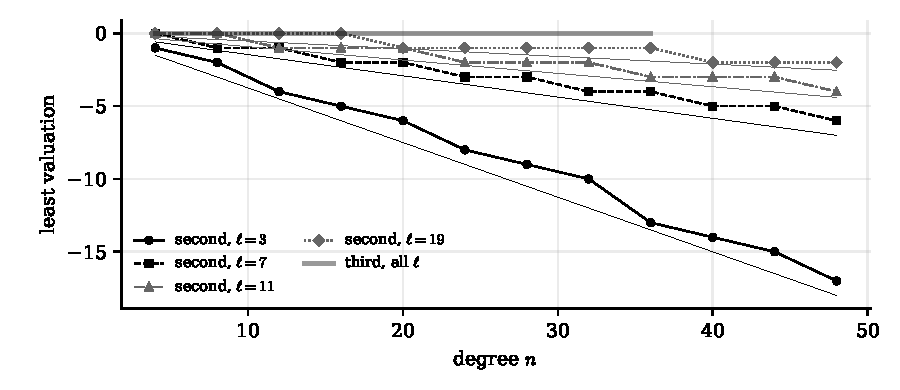
\includegraphics[width=0.95\textwidth]{fig/mq_differences_ag.pdf}
\caption{Least valuation of the coefficients of degree $n$ in formal coordinates at an inert prime $\ell$ (exact computation): the second difference loses about $n\ell/(\ell^2-1)$ (thin lines), the third difference is integral (grey line at $0$).}\label{mqg:fig:differences}
\end{figure}

In Figure~\ref{mqg:fig:differences} the second difference of $\log(\sigma/t)$ has $\ell$ adic denominators growing, as an empirical guide, like $n\ell/(\ell^2-1)$ in degree $n$, and the third difference, the series $\exp(\Delta_1\tilde\beta)$ of Step 1 (unprojected; the theorem concerns the projection $\beta$), is integral in every degree computed (up to $36$).

\begin{remark}[abstract form]\label{mqg:rem:abstract}
The proof uses a power series $m$ on a space $V=V_{\rm ev}\oplus V_{\rm od}$ with logarithmic coordinates on a product of formal groups over an unramified ring, a finite group $G$ of order prime to $\ell$ acting on $V$ through formal automorphisms preserving the decomposition, inclusions of $V_{\rm ev}$ and $V_{\rm od}$ that are themselves integral formal subgroup maps, and integrality of the exponential of the cube of $m$ on $V$. Under these hypotheses the same three steps give the integrality of $\exp(\Delta_1\beta)$ for the invariant part $\beta$ of $m(z+w)-m(z)-m(w)$, $z\in V_{\rm ev}$, $w\in V_{\rm od}$. Whether such data exist for orbits of longer length is open, we make no claim for them, and the local table of the Rubinstein draft (the minimum valuations of $\exp(\Delta_1\beta)$ by degree) is not reproduced: some of its exact degree entries are wrong (for $\ell=7$ no invariant monomial of total degree $4$ exists, so the degree four part of $\exp(\Delta_1\beta)$ vanishes).
\end{remark}

\subsection{Comparison with the Rubinstein draft}

We compared the above with the working draft \cite{Rub26}, of which we read Part I and the statement of the central hypothesis. As reported, and unverified here: that draft does not prove (M), derives RH from (M) and two estimates, works with derivatives of theta series of Hermitian lattices over a CM field with Gaussian size and divisibility at inert primes. Our computations are consistent with the corresponding statements on the divisibility side (Conjecture~\ref{mqg:conj:sigma}) and do not test the rest. A computation of the second difference $\sigma(z+w)zw/(\sigma(z)\sigma(w)(z+w))$ for the lemniscatic lattice gives at the single bidegree $(36,36)$ a value of Gaussian size ($\log|N_{36,36}|=120.28$ against $\frac12\log72!=119.49$, with $N_{36,36}=a!\,b!$ times the coefficient at $a=b=36$) and inert primes carrying $12.68$ of the logarithm (the primes $p\equiv3\pmod4$ up to $72$). This establishes neither Gaussian growth of the series nor the divisibility requirement of the draft, and is not a test of (B4): the series is not the invariant part, and the normalisation is by $z$, not by the formal parameter.

